\begin{illustration}{packages}

\tikzset{
  rect/.style={draw,fill=green!15,minimum height=0.8cm,rectangle},
  box/.style={
    draw=blue!50!white,
    line width=1pt,
    dash pattern=on 1pt off 4pt on 6pt off 4pt,
    inner sep=4mm, rectangle, rounded corners
  },
}

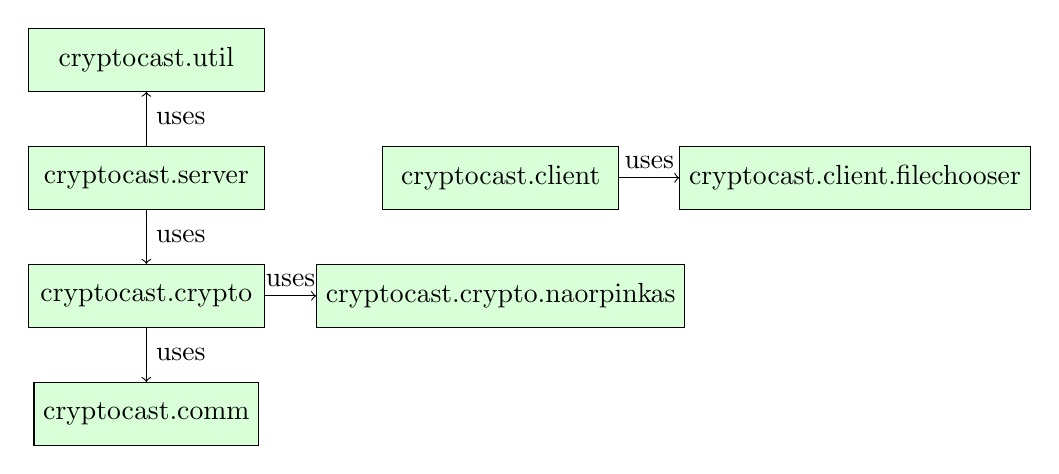
\begin{tikzpicture}[auto,node distance=1.5cm]

\node[rect,minimum width=3cm](util) {cryptocast.util};
\node[rect,minimum width=3cm, below of=util](server) {cryptocast.server};
\node[rect,minimum width=3cm, xshift=3cm, right of=server](client) {cryptocast.client};
\node[rect,minimum width=3cm, xshift=3cm, right of=client](file) {cryptocast.client.filechooser};
\node[rect,minimum width=3cm, below of=server](crypto) {cryptocast.crypto};
\node[rect,minimum width=3cm, xshift=3cm, right of=crypto](naor) {cryptocast.crypto.naorpinkas};
\node[rect,minimum width=2cm, below of=crypto](comm) {cryptocast.comm};

\draw [<-] (util.south) -- ( server.north)
             node[pos=.5]{uses};

\draw [->] (server.south) -- (crypto.north)
             node[pos=.5]{uses};
\draw [->] (crypto.south) -- (comm.north)
             node[pos=.5]{uses};
\draw [->] (crypto.east) -- (naor.west)
             node[pos=.5]{uses};
\draw [->] (client.east) -- (file.west)
             node[pos=.5]{uses};

\end{tikzpicture}

\end{illustration}